\documentclass{san-g}
\begin{document}

\section{Summary of the trail system of the San Gorgonio Wilderness}

\vspace{10mm}

\includegraphics{figs/schematic}

The water drop symbol indicates a water source. Some of these may not run year-round or
in dry years.

\vspace{10mm}

\begin{tabular}{lp{30mm}l}
                 & \emph{miles to the}  \\
                 & \emph{summit}  \\
\emph{trailhead} & \emph{(round trip)} & \emph{climb factor${}^*$} \\
Vivian Creek                 &   17.1   &   25\% \\
South Fork via Dollar Lake   &   19.2   &   17\% \\
South Fork via Dry Lake      &   21.2   &   15\% \\
Forsee                       &   24.0${}^{**}$   &   20\% \\
Momyer                       &   25.4   &   24\% \\
Angelus Oaks                 &   32.5   &   17\% 
\end{tabular}

${}^*$ \scriptsize{The climb factor is an estimate of the additional calories you burn
in order to do this route, versus if the route was flat.
It's a more meaningful figure than elevation gain, because for
out-and-back or loop routes that aren't extremely steep, the energy conserved on
downhills comes close to canceling out the extra energy expended on climbing. For more
info about how the climb factors were calculated, and how to calculate
a climb factor from a GPS track, see \url{github.com/bcrowell/kcals}. The elevation gain for
these routes varies from 4500 to 7500'.
}
${}^{**}$ \scriptsize{Other sources estimate this at over 30 miles. I don't know the reason
for the discrepancy, which seems to be partly because they estimate a longer distance
for the segment leading up to Dollar Lake Saddle.
}

\vspace{10mm}

\normalsize For more detailed information about trails, water sources, and camping, see \url{sgwa.org}.
This schematic is only for use as an overview for planning trips. Don't use it as a substitute
for a real map. USGS topo maps are available for free from \url{store.usgs.gov/map-locator}.

\vfill

\myfooter
\end{document}
